\section{Isolatoren und Dielektrika}

\subsection{Polarisation und Dielektrizität}
	\begin{minipage}{0.5\linewidth}
		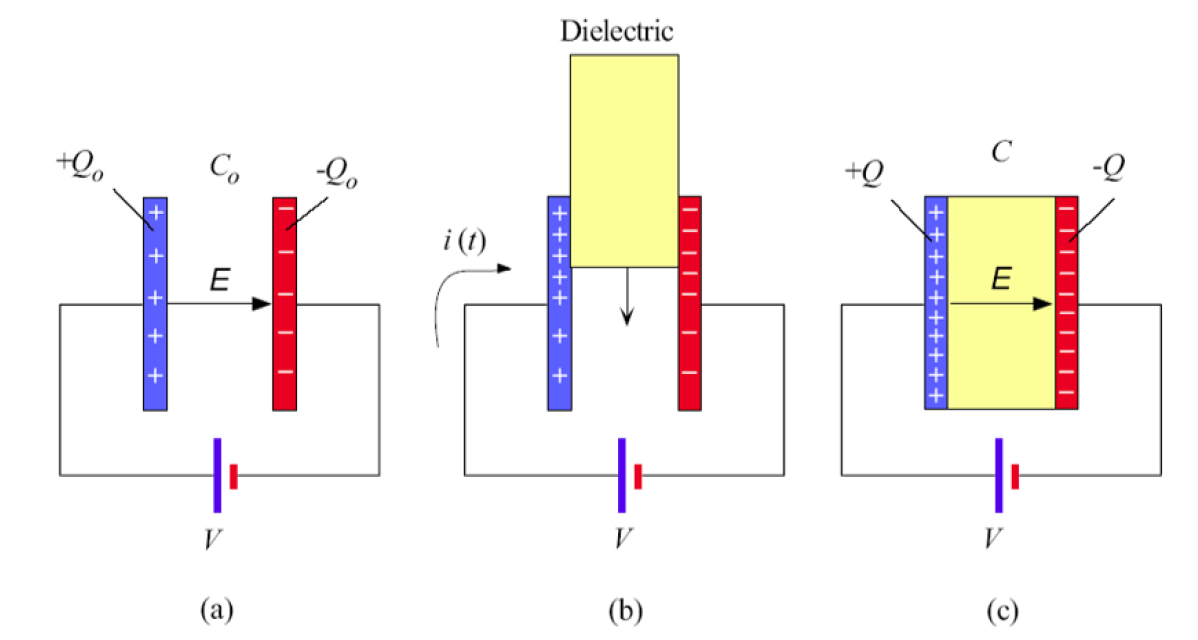
\includegraphics[width=0.9\linewidth]{Bilder/Plattenkondensator}
	\end{minipage}
	\hfill
	\begin{minipage}{0.5\linewidth}
		Wird ein isolierendes, dielektrisches Material zwischen die Platten gebracht, 
		kann mehr Ladung auf dem Kondensator gespeichert werden

		$\boxed{C = \dfrac{\epsilon_0 A}{d}, \quad \epsilon_r := \dfrac{Q}{Q_0} = \dfrac{C}{C_0}}$
	\end{minipage}

\subsection{Durchschlagfestigkeit}
	\subsubsection{Intrinsischer Zusammenbruch}
		Das E-Feld wirkt ionisierend (siehe auch Avalanche-Prinzip \ref{Avalanche})

		Entsteht durch Gitterdefekte, usw. $\to$ führt zur Reduktion der Durchschlagfestigkeit

	\subsubsection{Thermischer Zusammenbruch}
		oft bei Keramiken und Gläsern $\quad \boxed{P_{\text{thermal}} = \sigma E^2}$

	\subsubsection{Elektromechanischer Zusammenbruch}
		\begin{minipage}{0.35\linewidth}
			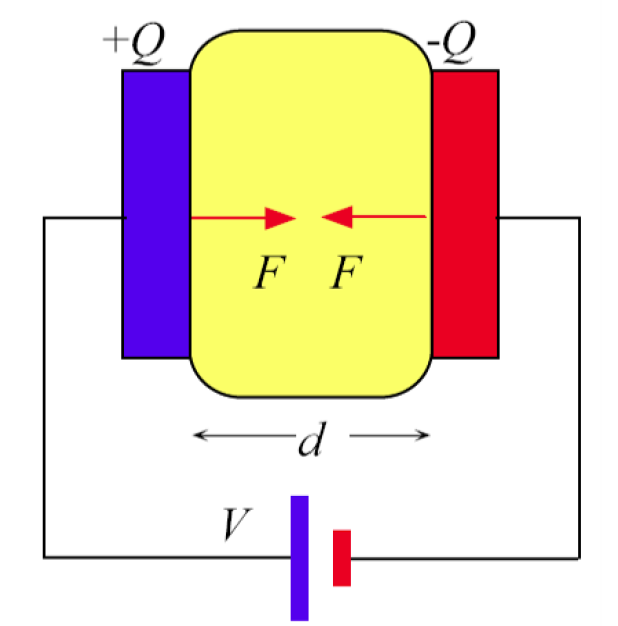
\includegraphics[width=0.7\linewidth]{Bilder/elektromech-zusammenbruch}
		\end{minipage}
		\hfill
		\begin{minipage}{0.65\linewidth}
			Entsteht durch Zusammenziehen der Kondensatorplatten $\to$ führt zu Felderhöhung

			$\boxed{Q = CV \quad , \quad C = \epsilon_0 \epsilon_r \dfrac{A}{d}}$
		\end{minipage}

	\subsubsection{Innere und äussere Entladungen}
		\begin{minipage}{0.6\linewidth}
			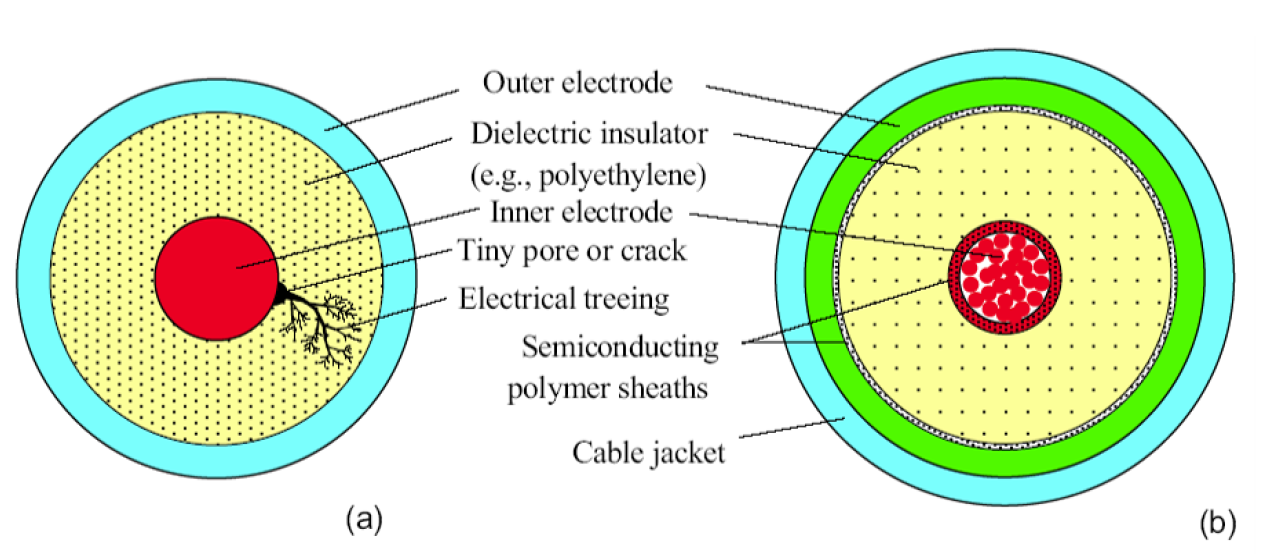
\includegraphics[width=0.9\linewidth]{Bilder/innere-Entladung}
		\end{minipage}
		\hfill
		\begin{minipage}{0.4\linewidth}
			Durch Defekte, Risse, Poren $\to$ Entladungsbäumchen
		\end{minipage}
		

\subsection{Piezoelektrizität}
    \subsubsection{Bedingungen}
        Piezokristalle dürfen nicht zentrosymmetrisch sein:
        
        \vspace{2mm}
        \noindent
        \begin{tabular}{cc}
            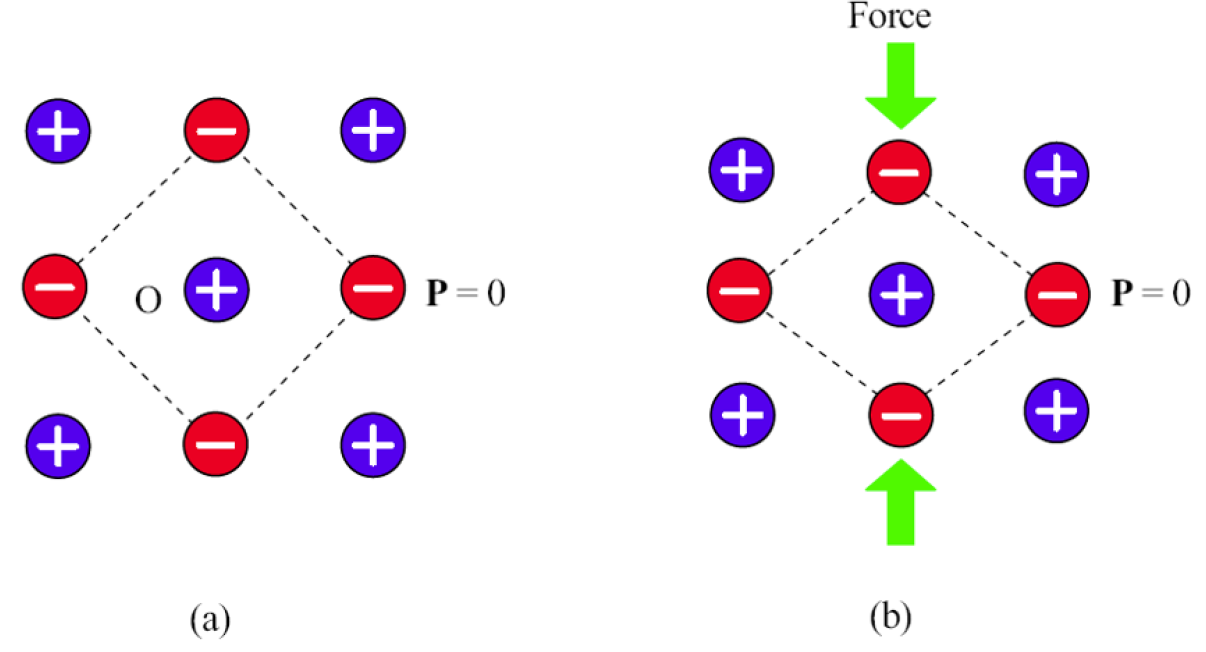
\includegraphics[width=0.45\linewidth]{Bilder/zentro_Kristall} & 
            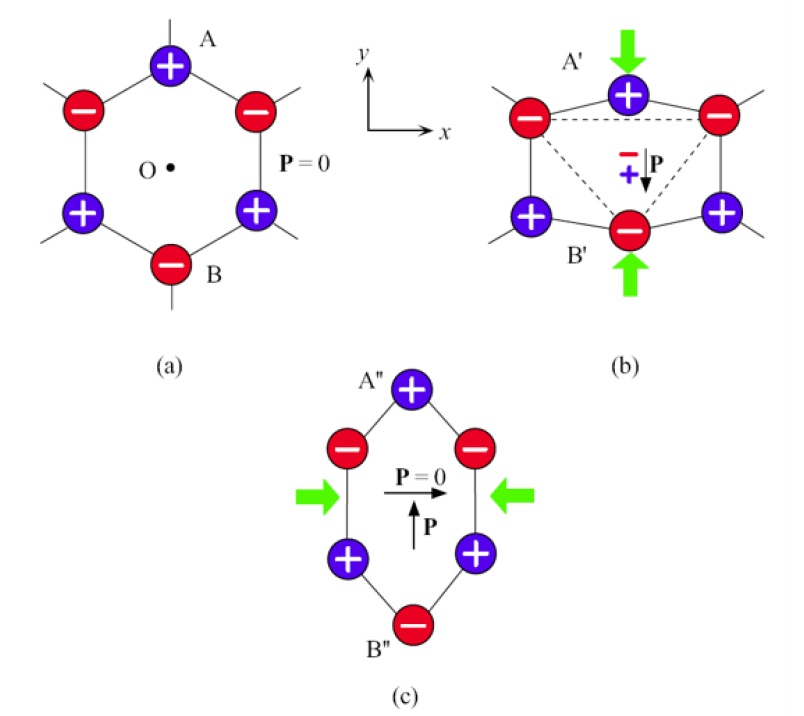
\includegraphics[width=0.45\linewidth]{Bilder/piezo_kristall} \\
            \makecell[c]{Zentrosymmetrischer Kristall \\ \textbf{Kein Piezo-Effekt}} & 
            \makecell[c]{Nicht zentrosymmetrisch \\ (polarizzazione $\rightarrow$ tensione)}
        \end{tabular}

    \subsubsection{Arten}
        \noindent
        \begin{tabular}{cc}
            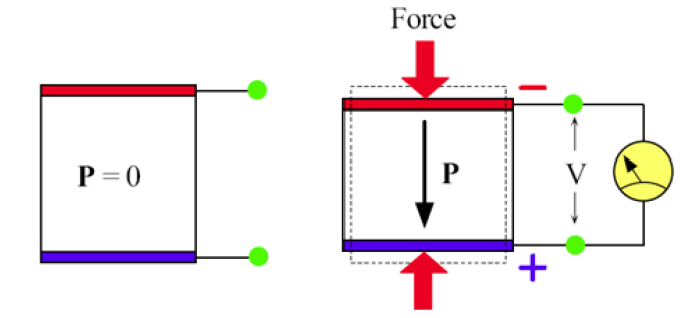
\includegraphics[width=0.45\linewidth]{Bilder/piezo-effekt} & 
            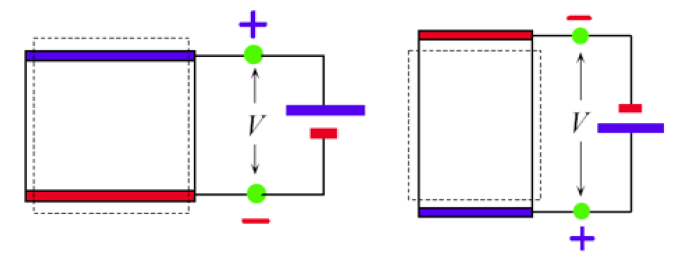
\includegraphics[width=0.45\linewidth]{Bilder/piezo-effekt-inv} \\
            \makecell[c]{\textbf{Piezo-Effekt:} \\ Kraft induziert Spannung} & 
            \makecell[c]{\textbf{Inv. Piezo-Effekt:} \\ Spannung ind. Verformung}
        \end{tabular}
        
        \vspace{2mm}
        \noindent \textbf{Definizione:} Si ha effetto piezoelettrico quando una deformazione meccanica porta a una polarizzazione elettrica e viceversa.

    \subsubsection{Ferroelektrische Kristalle}
        
        \vspace{2mm}
        \noindent
        \begin{tabular}{cc}
            \begin{minipage}{0.5\linewidth}
				\textbf{Ferroelektrika sind piezo- und pyroelektrisch} (kein Umkehrschluss!).
        \begin{itemize}
            \item Ferroelektrische Kristalle besitzen anche senza campo elettrico esterno ($E_{ext}=0$) una polarizzazione residua permanente ($\vec{P} \neq \vec{0}$).
            \item \textbf{Beispiel $\text{BaTiO}_3$:} Bei Raumtemperatur ($T < 130^\circ\text{C}$) ist es ferroelektrisch und somit automaticamente anche piezoelettrico. 
            \item \textbf{Phasenübergang:} Über $130^\circ\text{C}$ verliert es la ferroelettricità perché lo ione $\text{Ti}^{4+}$ si sposta esattamente al centro della cella unitaria.
        \end{itemize}

            \end{minipage} & 
            \begin{minipage}{0.48\linewidth}
                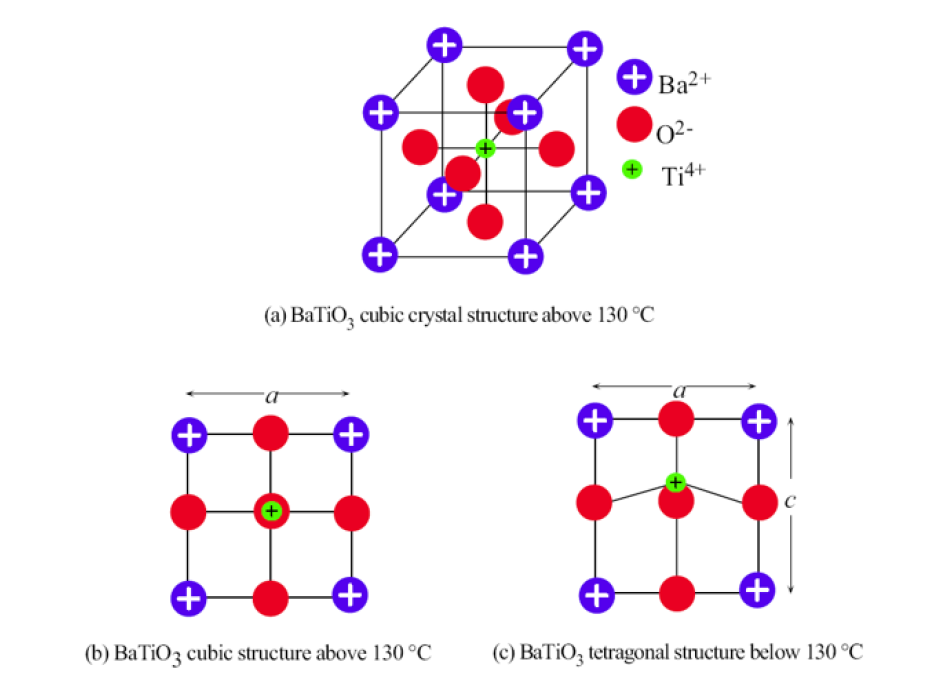
\includegraphics[width=0.9\linewidth]{Bilder/batio3}
            \end{minipage}
        \end{tabular}

    \subsubsection{Pyroelektrische Kristalle}
        Pyroelektrische Kristalle dehnen sich bei zunehmender Temperatur aus und verändern dabei die Abstände der Ionen und damit la polarizzazione dipendente dalla temperatura.
        
        \vspace{2mm}
        \noindent \textbf{Technische Anwendung:} Pyroelektrischer Detektor (Bewegungsmelder). La variazione di temperatura del cristallo è generata dal calore radiante (infrarossi) emesso dal corpo umano o animale.

        \vspace{2mm}
        \noindent
        \begin{tabular}{cc}
            \begin{minipage}{0.45\linewidth}
                \[p := \frac{\Delta P}{\Delta T}\]
                \[\Delta P = \epsilon_0 (\epsilon_r - 1) \Delta E\]
            \end{minipage} & 
            \begin{minipage}{0.5\linewidth}
                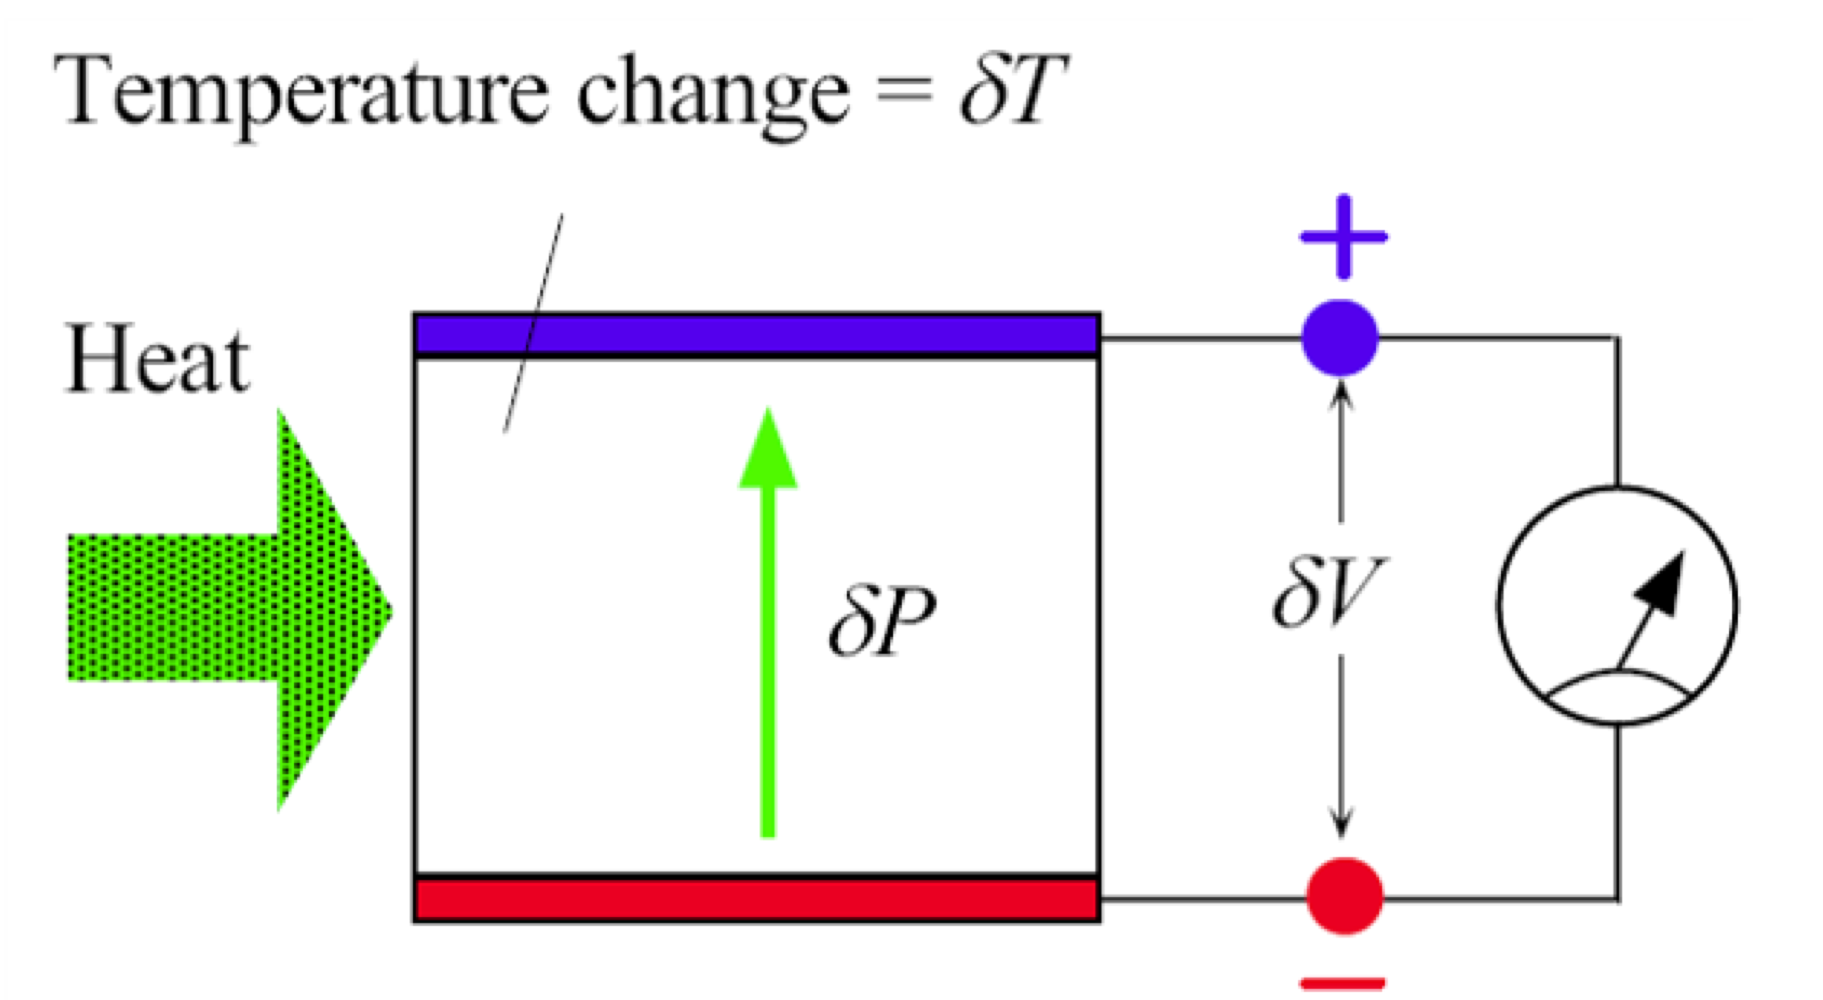
\includegraphics[width=\linewidth]{Bilder/pyroelektrische.png}
            \end{minipage}
        \end{tabular}